En el presente trabajo mejoramos el modelo original pasando de un AUC de 0.74 a 0.90. Pero además hemos explorado diferentes aristas relativas al problema de predicción planteado con el objetivo de responder nuestros interrogantes iniciales. 

La primera pregunta era acerca de la posibilidad de enriquecer el dataset VarQ con nuevas fuentes de datos. Esta pregunta fue respondida afirmativamente, dado que agregar nuevas dimensiones demostró ser efectivo en la mejora del modelo, manteniendo fijo el algoritmo utilizado, siendo este Random Forest en todos los casos. En particular, el modelo que usó variables genómicas, arrojó un AUC de 0.85. El otro conjunto de variables analizado, las Físico-Químicas alcanzaron un AUC de 0.72. Si bien el AUC no fue superior al del modelo VarQ Curado, este demostró ser de utilidad. El modelo Integral, que combinó ambos datasets, resultó ser mejor que los dos anteriores, llegando a un AUC de 0.88 (figura \ref{fig:curvas_auc_humsavar}). Por último, sumar estas variables al dataset VarQ Curado también mostró una mejora, pasando de un AUC de 0.74 a 0.86 (figura \ref{fig:curvas_auc_varq}). 

La segunda pregunta que nos hicimos al comienzo del trabajo era sobre cómo la las variables afectan a nuestros modelos. La descripción estadística del dataset nos permitió entender como el método estándar para calcular importancia de variables en métodos de ensamble se ve afectado en variables altamente correlacionadas. Con respecto a las variables utilizadas, detectamos que las variables de conservación (phastCons y phyloP) son las más relevantes para nuestro problema de predicción. Si bien el dataset VarQ ya poseía variables de conservación, estas pertenecen a familias de proteínas (Pfam). Otras variables de importancia considerable son la variación de la energía (del dataset VarQ, obtenida vía PDB) y las matrices de sustitución o distancia (GRANTHAM, PAM250, BLOSUM, EX, JM y VB). Un aspecto destacable es que esta lista de variables corresponden a datasets distintos, reforzando la conclusión sobre la importancia de sumar dimensiones al problema.

Este trabajo también consistió en una comparación de distintos métodos de aprendizaje automático. En la primera sección del desarrollo comparamos tres métodos clásicos con el dataset VarQ Curado: Regresión Logística, Support Vector Classifier y Random Forest, obteniendo mejores resultados con éste último. Luego en la última sección del trabajo comparamos Random Forest con un método más avanzado de ensamble, XGBoost en los datasets Integral, mejorando la performance del modelo de un AUC de 0.88 a 0.90; y VarQ+Integral, llevando el AUC de 0.86 a 0.88.

\section{Trabajo Futuro}

Uno de los principales productos de este trabajo es la generación de un nuevo dataset que contiene numerosas variables estructurales y físico-químicos de la proteína, sumados a variables de tipo genómico. Este dataset también contiene variantes que están ligados a diferentes genes, que a su vez poseen cantidades distintas de SNPs potencialmente dañinos. Una de los trabajos que quedaron pendientes consisten en generar modelos individuales para cada gen, dado que puede existir un sesgo en nuestro modelo en caso de tener un número muy grande de SNPs de un gen determinado. También creemos que los trabajos futuros que deriven de este deberían hacer énfasis en la generación de modelos que mejoren la selección de hiperparámetros (en particular sugerimos el uso de técnicas de optimización bayesiana), y un tratamiento de nulos en variables categóricas más avanzado en comparación al usado en este trabajo. 

\begin{figure}[H]
\centering
\begin{subfigure}[b]{0.6\textwidth}
    \centering
    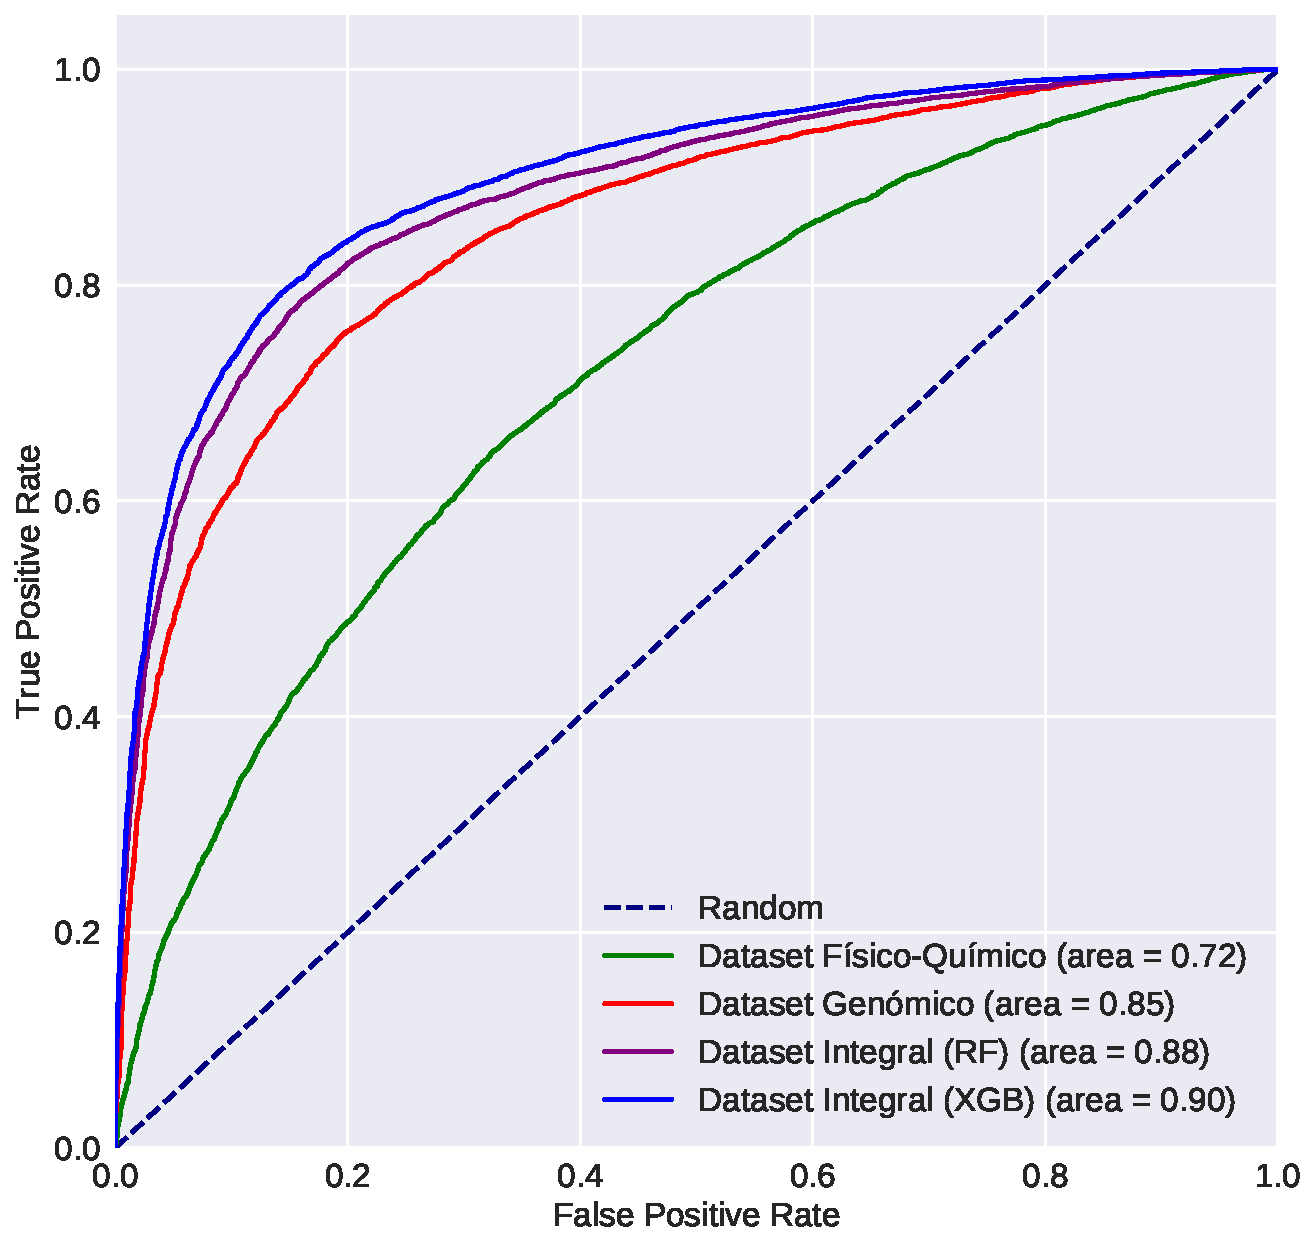
\includegraphics[width=\textwidth]{documents/latex/figures/4/curvas_auc_humsavar.pdf}
    \caption{Comparación de curvas ROC entre los datasets Físico-Químico, Genómico e Integral.}
    \label{fig:curvas_auc_humsavar}
\end{subfigure}

\hfill
\hfill

\begin{subfigure}[b]{0.6\textwidth}
    \centering
    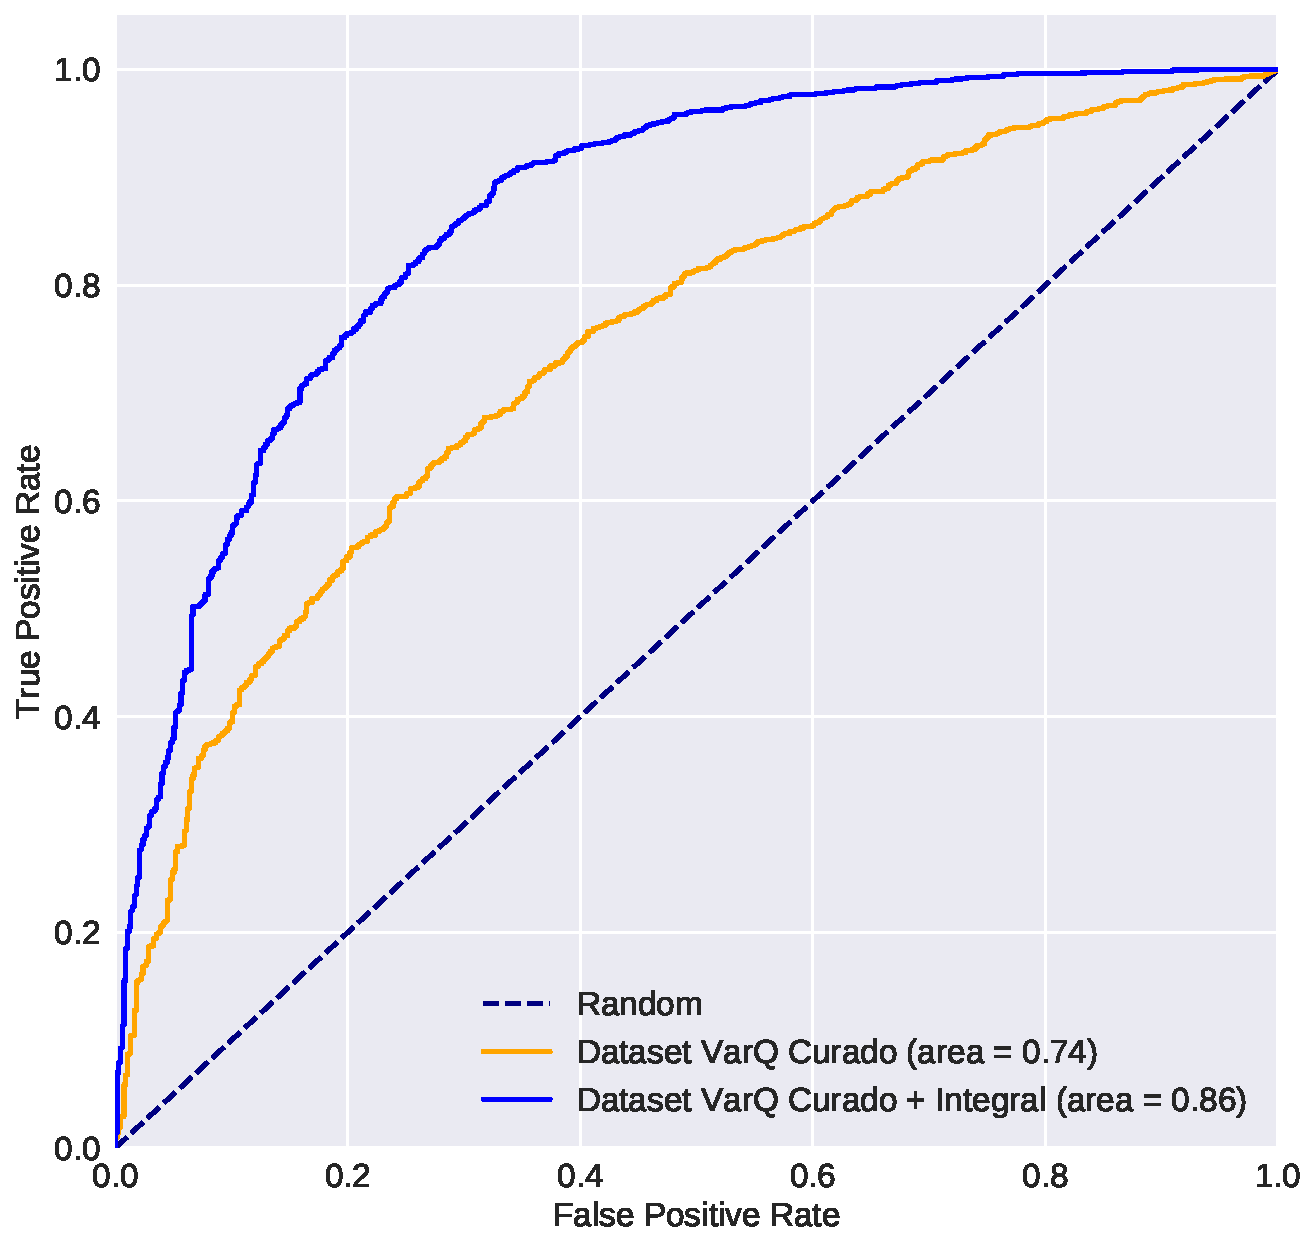
\includegraphics[width=\textwidth]{documents/latex/figures/4/curvas_auc_varq.pdf}
    \caption{Comparación de curvas ROC entre los datasets VarQ Curado y VarQ Curado + Integral.}
    \label{fig:curvas_auc_varq}
\end{subfigure}

\caption{Comparación de curvas AUC usando datasets con variantes de Humsavar y VarQ Curado.}
\end{figure}


